\chapter{Manual Annotation} \label{chapter:image_pose_annotation}

\begin{figure}[!tbp]
	\centering
    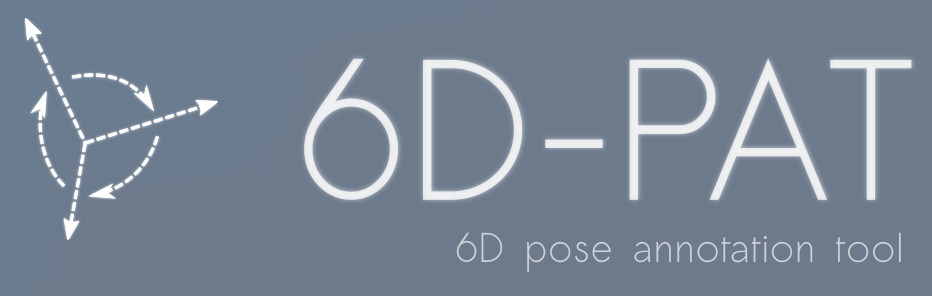
\includegraphics[width=\linewidth]{6dpat}
    \caption{The logo of the pose annotation tool 6D-PAT. Own image.}
    	\label{fig:6dpat_logo}
\end{figure} 

The following chapter analyzes manual 6D pose annotation process and its prerequisites. To this end, the necessary terminology is defined and explained and the workflow to annotate poses using the developed annotation tool is described. The assessment of the requirements of the annotation procedure and the creation of the tool are conducted based on the medical image dataset, which is described further below.

\section{Terminology} \label{section:terminology}

\textbf{Image.} An image $I$ is a 2D matrix of pixels. The pixel $u$ at position $(i, j)$ is referenced by the tuple $(x, y)$, where $x = j$ and $y = i$. The inverted notation is chosen over the common row-major matrix indexing to account for the universal  \\

\noindent\textbf{Object Model.} An \textit{object model}, or \textit{3D model}, $O$ is composed of a set of points $M \subseteq \mathbb{R}^3$ and a set of triangles $T = \{(m_1, m_2, m_3) \in M^3\}$. The real-world entity that the object model resembles is not restricted. In case of the T-Less dataset \cite{tless} the objects are mainly hardware like screws and power sockets. \\

\noindent\textbf{6D Pose.} A \textit{6D pose} $P$ is the tuple $(R, t)$, where $R$ is the 3x3 rotation matrix and $t$ the translation vector used to transform the respective object model into camera coordinates (see section \ref{objectcoordinates} for details). \\

\noindent\textbf{Correspondence.} A \textit{correspondence} $C$ is the tuple $(u, p)$, which captures the relation between a pixel $u$ of an image $I$ and an object model $O$. The pixel $u$ is the projection of the 3D point $p$ onto the image plane using the camera matrix $K$ and a pose $P$. If the pose is unknown, a set of at least three correspondences can be used to retrieve the pose computationally (see section \ref{objectcoordinates} for details). \\

\noindent\textbf{Segmentation Mask.} A \textit{segmentation mask} (or \textit{segmentation image}) $S$ for an image $I$ is a second image of the same size. Each position $(x, y)$ of the mask encodes the class of the pixel at $(x, y)$ in $I$. The set of classes can be defined arbitrarily. In the context of this work each class represents a type of object model. The segmentation mask can be seen as the mapping $s(x, y) = q_i$ for a class set $Q = \{q_0, \cdots, q_n\}$. \\

\noindent\textbf{Pose Creation.} The process of creating correspondences can be performed in various ways. In this work the key operation is to create a set of correspondences and solve the implied perspective-n-point problem. \\

\noindent\textbf{Ground-Truth.} A \textit{ground-truth pose} $\bar{P}$ is a 6D pose. A ground-truth pose is always created by a human instead of a machine. The ground-truth pose is the best approximation of the rotation and translation of an object model $O$ on an image $I$ of said object. It is an approximation because there can be a discrepancy between the real world object and its digital 3D representation. Distortions by the camera used to photograph the object and other influences might also not be modeled correctly or not accounted for at all. The rotation and translation error of a ground truth pose are bearable and thus are the objective for neural networks. \\

\noindent\textbf{Bindings.} \textit{Bindings} is the term for a set of code that allows code written in one language being used in a different one. \\

\noindent\textbf{Makefile.} A \textit{makefile} is the directive file used by the program \textit{make} to compile programs of any kind. Often more complex programs imply dependencies which have to be compiled in a certain order. This is an example what make takes care of and what is defined in a makefile. \\

\noindent\textbf{Training.} \textit{Training} stands for the process of training the neural network using gradient-descent (see chapter \ref{chapter:background}). \\

\noindent\textbf{Inference.} After training a neural network it can be used to infer poses on unseen images. This is called \textit{inference}.

\section{Medical Images}

The goal of this work is to provide a system to successfully and efficiently annotate the medical images that were provided upfront. The dataset includes segmentation masks but no object models or existing pose annotations. An example image together with the corresponding segmentation mask are given in fig \ref{fig:sfb}. The dataset resembles the characteristics and quality of images from laparoscopic videos, i.e. there is no depth information present and occlusion and artifacts like motion blur can occur. The issues with this dataset are discussed in section \ref{section:6dpat_difficulties}. 

\begin{figure}[!tbp]
	\centering
	\begin{subfigure}[t]{0.47\textwidth}
	\centering
    	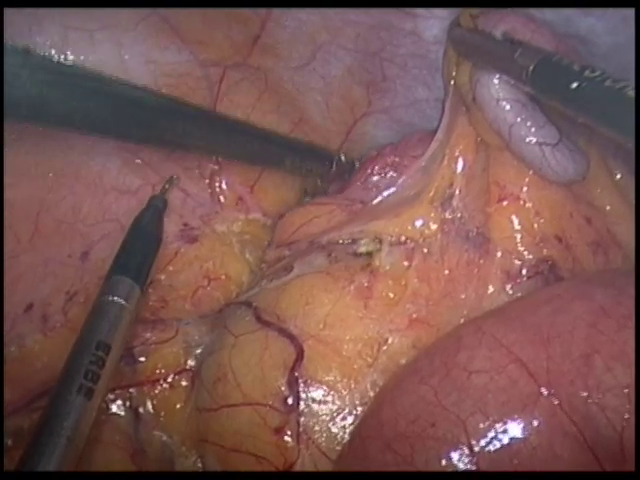
\includegraphics[width=0.8\linewidth]{sfb_original}
    	\caption{An example image from the medical dataset. Taken from TODO: cite.}
    	\label{fig:sfb_original}
	\end{subfigure}
	\hfill
	\begin{subfigure}[t]{0.47\textwidth}
	\centering
    	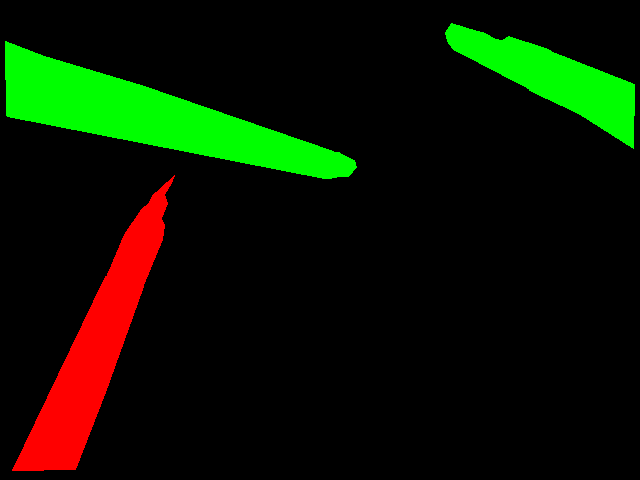
\includegraphics[width=0.8\linewidth]{sfb_segmentation}
    	\caption{The corresponding segmentation mask to the image in fig \ref{fig:sfb_original}. The colors encode the tools' classes. Taken from TODO: cite.}
    	\label{fig:sfb_segmentation}
	\end{subfigure}
	\caption{An example image and its corresponding segmentation mask from the medical dataset.}
	\label{fig:sfb}
\end{figure} 

\section{6D Pose Annotation Tool (6D-PAT)}

The creation of sufficient training data for neural networks can be a time-consuming and tedious process. Using non-specialized tools designed for other purposes, like 3D modeling programs, require the annotation personnel to get accustomed to complex user interfaces (UIs). The goal of the annotation tool is to provide a system that allows easy and efficient annotation of images, images of the medical dataset in particular. The annotated poses, the so-called \textit{Ground-Truth Poses} (see section \ref{section:terminology}), can later be used to train a neural network. The program is written in the language C++ and named \textit{6D - Pose Annotation Tool (6D-PAT)}. Its logo can be seen in fig \ref{fig:6dpat_logo}. Although the program was developed using the \textit{Linux}-based operating system \textit{Ubuntu}, it is compilable on other systems as well.

\subsection{Requirements}

TODO. \\

TODO. \\

TODO. \\

TODO. \\

TODO. \\

\subsection{Frameworks \& Third-Party Libraries}

The listed frameworks are all necessary dependencies of the annotation tool. There are no dependencies other than the mentioned ones. They are not part of the repository but have to be compiled individually instead. Since all three frameworks/libraries are platform-independent the program can be compiled and run on different systems. \\

\noindent\textbf{Qt.} \textit{Qt} \cite{qt} is a powerful framework for C++ that offers a vast selection of user interface components but also general functionality that exceeds the capabilities of the standard C++ library. Qt is also chosen as the main framework because it ensures portability of C++ applications by encapsulating system calls of all kind. The program \textit{Qt Creator} is the \textit{Integrated Development Environment (IDE)} that is included in the Qt distribution was used to write and execute the code of 6D-PAT. An IDE combines an editor to edit code an some environment to execute it. \\

\noindent\textbf{OpenGL.} \textit{OpenGL} \cite{opengl} is a widespread open-source 3D graphics library specification. Implementations for many operating systems exist, thus making most OpenGL using applications compilable in different environments without further modifications. \textit{Mesa 3D} \\

\noindent\textbf{OpenCV.} \textit{OpenCV} \cite{opencv} is a C++ library created for various computer vision tasks, hence the name. OpenCV provides implementations for tracking, object detection, segmentation and many more. In this work its \textit{solvePnPRansac} is used. \\

\noindent\textbf{Assimp.} \textit{Assimp} \cite{assimp} is a C++ library designed to import 3D models. The library was incorporated into the tool to ensure a broad support of 3D model formats.

\subsection{Architecture \& Code Design}

\begin{figure}[!tbp]
	\centering
	\begin{subfigure}[t]{0.47\textwidth}
		\centering
    	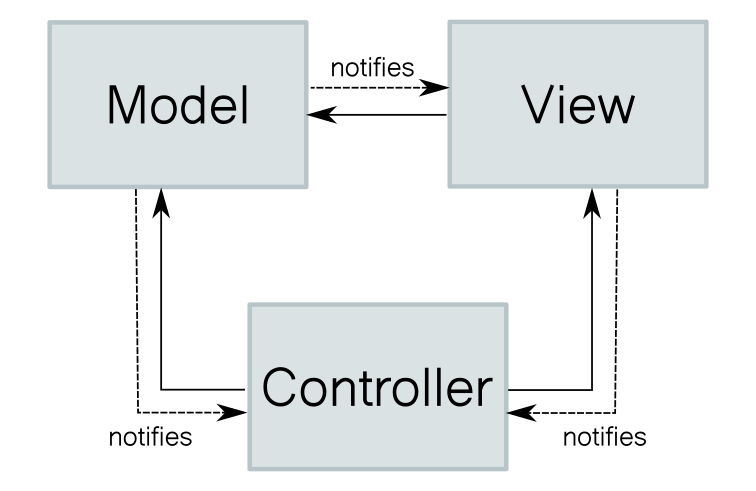
\includegraphics[width=0.8\linewidth]{mvc}
    	\caption{The Model-View-Controller architecture. The solid lines stand for a direct connection either because the target is owned or known by reference. The dashed line is an indirect connection using for example the observer pattern or the Qt Signals and Slots mechanism visible in fig. \ref{fig:qt_signals_slots}. Own image.}
    	\label{fig:mvc}
	\end{subfigure}
	\hfill
	\begin{subfigure}[t]{0.47\textwidth}
	\centering
    	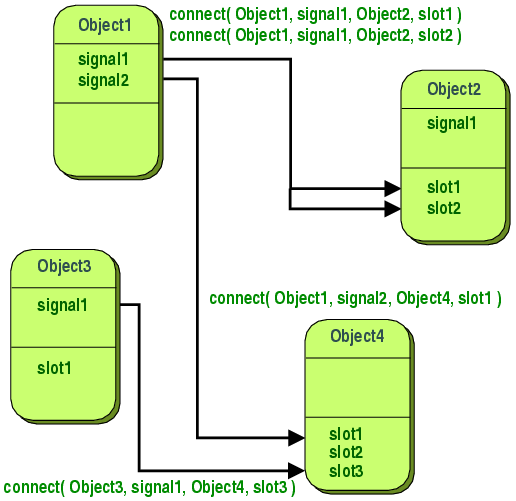
\includegraphics[width=0.8\linewidth]{qt_signals_slots}
    	\caption{The Signals and Slots mechanism of Qt. A class can define signals it can emit, independently of any listeners waiting for that signal. Slots are the functions that, when connected a signal, are called and can thus react to the signal. Image taken from \cite{qt_signals_and_slots}.}
    	\label{fig:qt_signals_slots}
	\end{subfigure}
	\caption{Two basic architectural concepts used in 6D-PAT: the model view controller pattern and the signal and slots pattern.}
\end{figure} 

6D-PAT is primarily a \textit{Graphical User Interface (GUI)} program primarily, i.e. its purpose is to display a window and enable optical interaction like clicking. Thus, the chosen underlying architecture is \textit{Model-View-Controller (MVC)}, which separates the concerns of data management (Model), displaying data (View) and high level logic (Controller). The schematic of the MVC architecture is given in fig. \ref{fig:mvc}. The indirect connections are realized via the Qt Signals and Slots mechanism, which is visualized in fig. \ref{fig:qt_signals_slots}. To speed up interface creation, \textit{Qt Designer} is used to layout the views. Qt Designer is a graphical tool that allows placement of UI components and linking of signals and slots. \\

TODO: describe class diagram first and then say what component is visible in the figure

The different sections highlighted in fig. \ref{fig:6dpat_components} are the main classes of the visual part of the program. Those components are the two breadcrumb navigations A and D, which show the currently selected folder to load images and object models from respectively. The loaded images can be viewed in gallery B and the loaded objects models in gallery E. An image that was selected from the gallery B is displayed in the \textit{Correspondence Viewer} dubbed window C at the bottom left. The view F is called the \textit{Correspondence Editor}. It's showing the selected object model and controls to edit existing correspondences. \\

The format that the program expects the image information file and the ground-truth poses file to be in is the \textit{JSON Format}. JSON is a format that is relatively easy for humans to read and is used by many deep learning applications. Transforming JSON formats can be done quickly and therefore provides the possibility to read data from other projects. \\

A Python bridge is included in the program to establish interoperability between the annotation tool and the neural network. This implies a more complex setup process to compile the program but is crucial to allow refining and developing the used neural network in Python, which is more common than implementing the network in C++. 

\begin{figure}[!tbp]
	\centering
    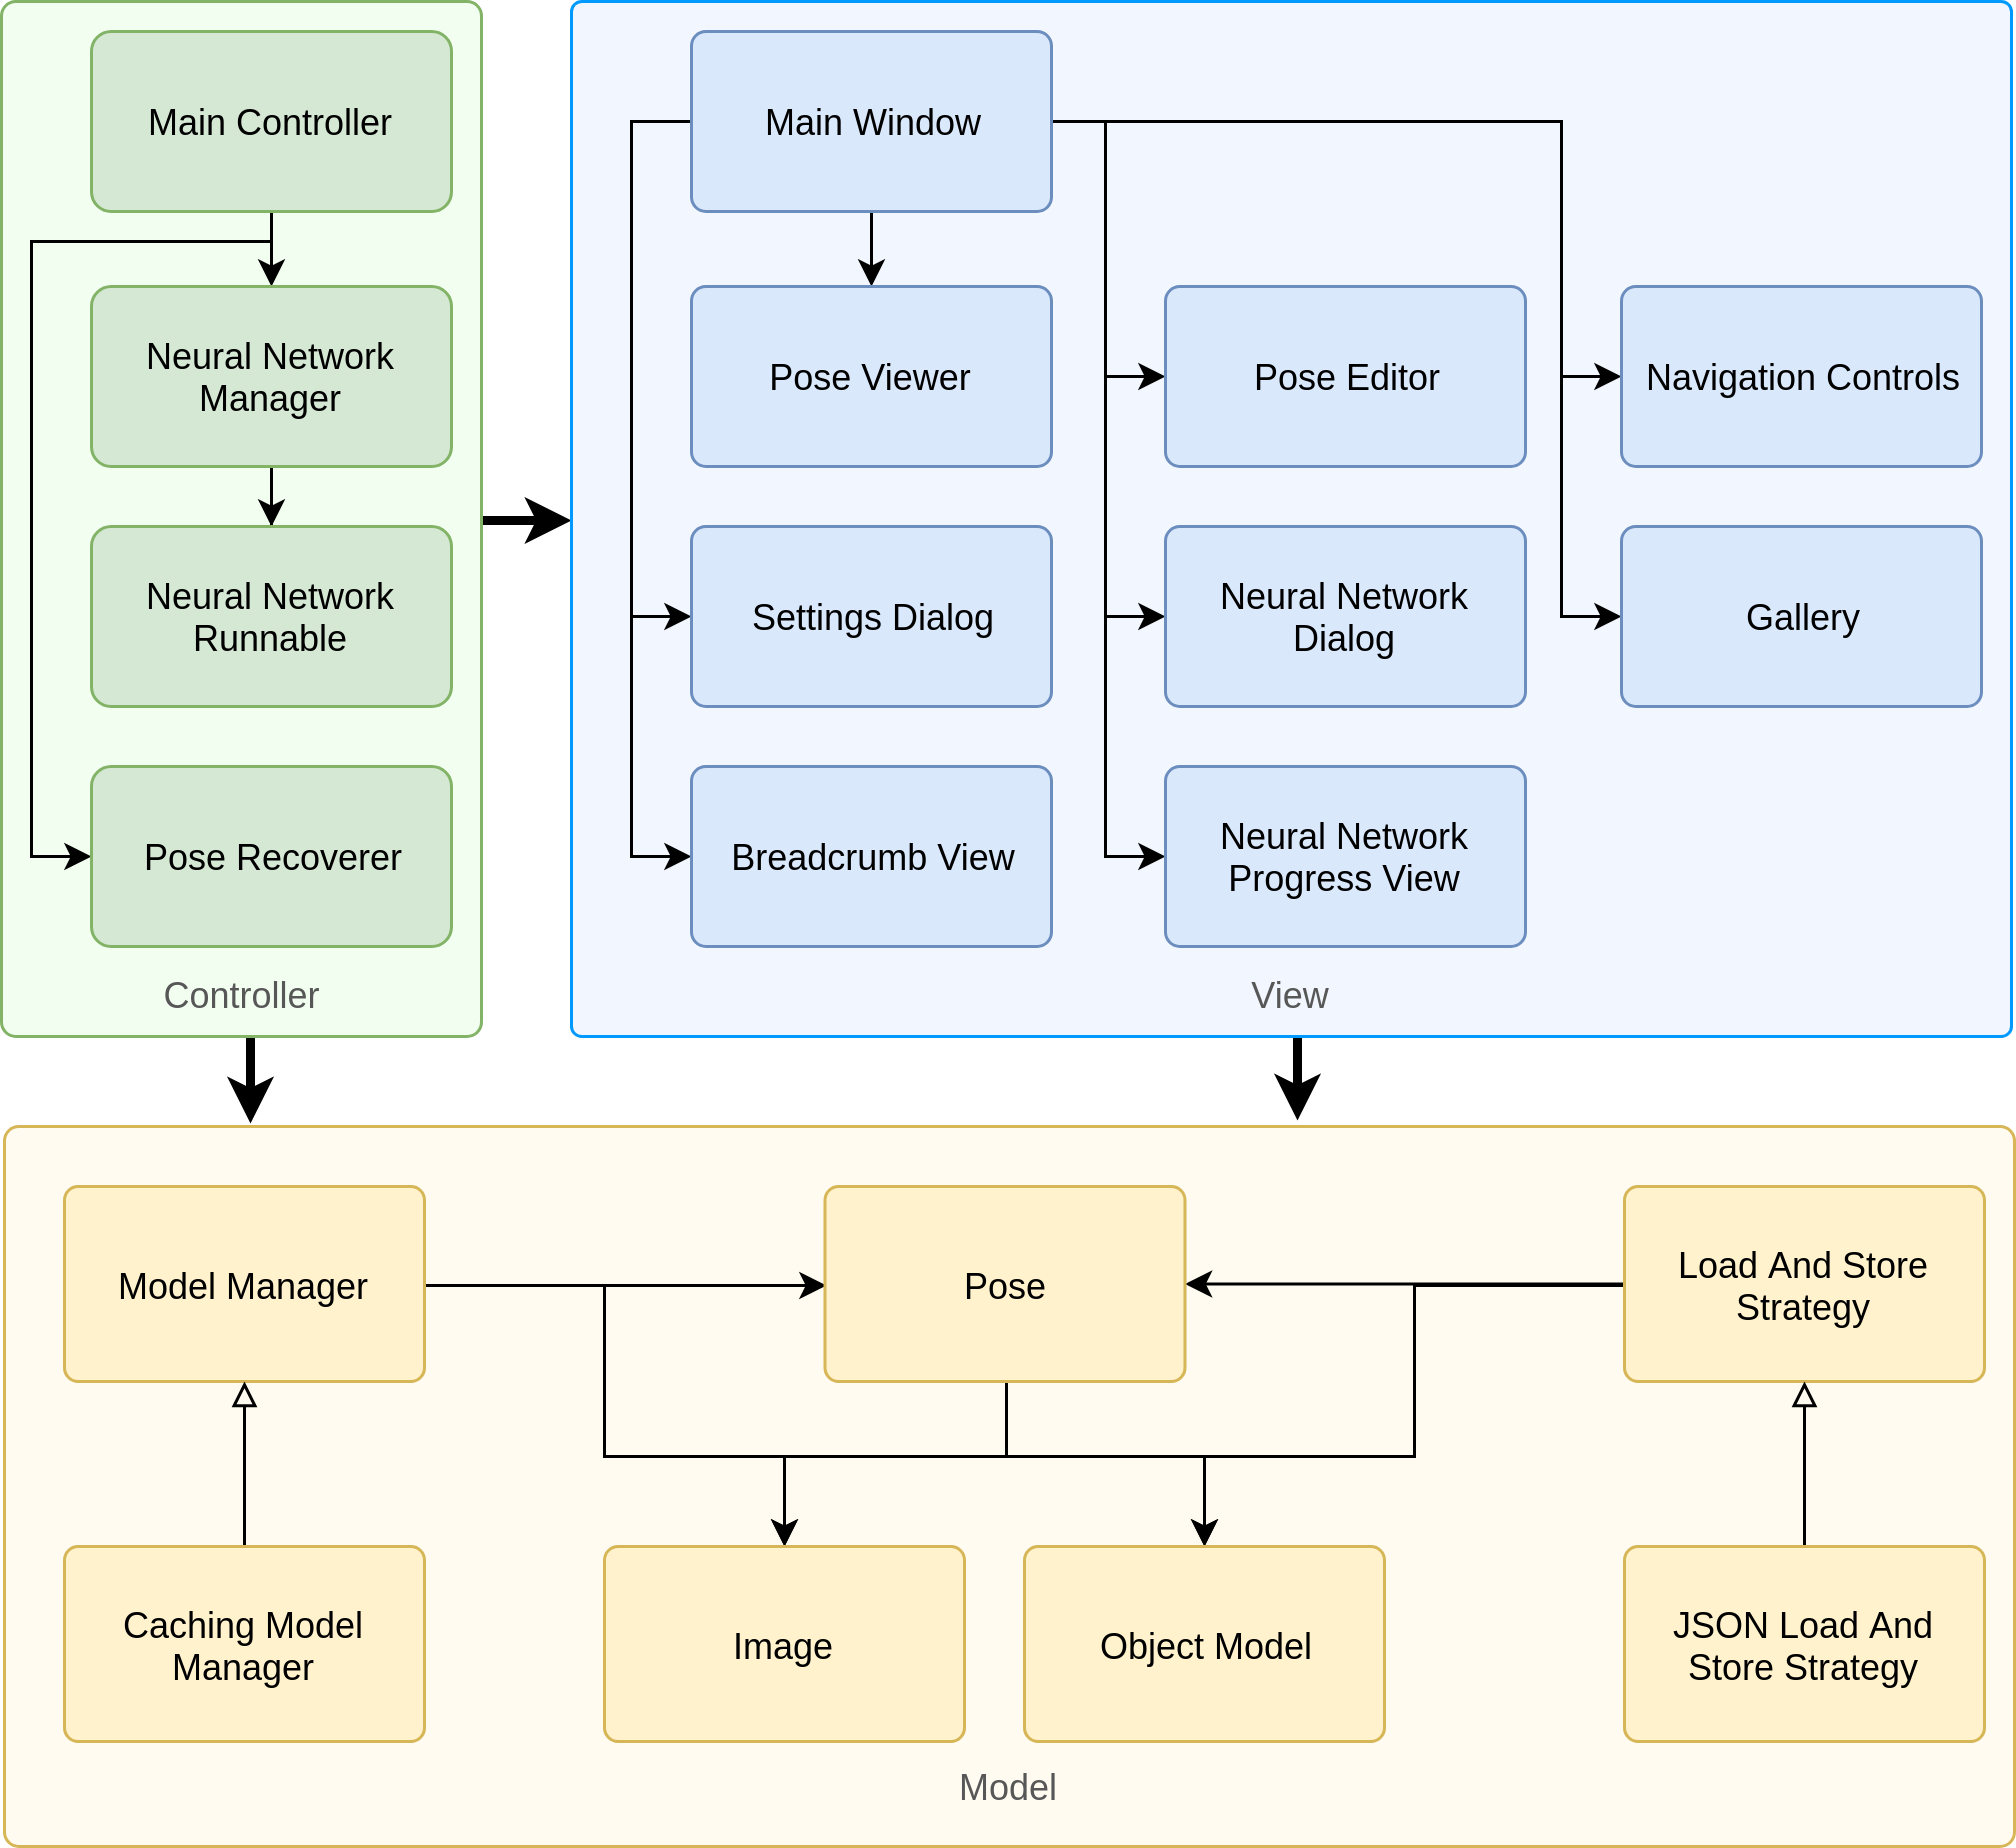
\includegraphics[width=\linewidth]{6dpat_class_diagram}
    \caption{An abstract high-level class diagram of the a subset of the classes of 6D-PAT. Own image.}
    \label{fig:6dpat_components}
\end{figure} 

\subsection{Manual Annotation} 

This sections describe the user interface of 6D-PAT and the required steps to annotate images with 6D poses. The process needs some actions performed before the actual annotation can be begin. 

\subsubsection{Preparation}

\begin{figure}[!tbp]
	\centering
	\begin{subfigure}[t]{\textwidth}
		\centering
    	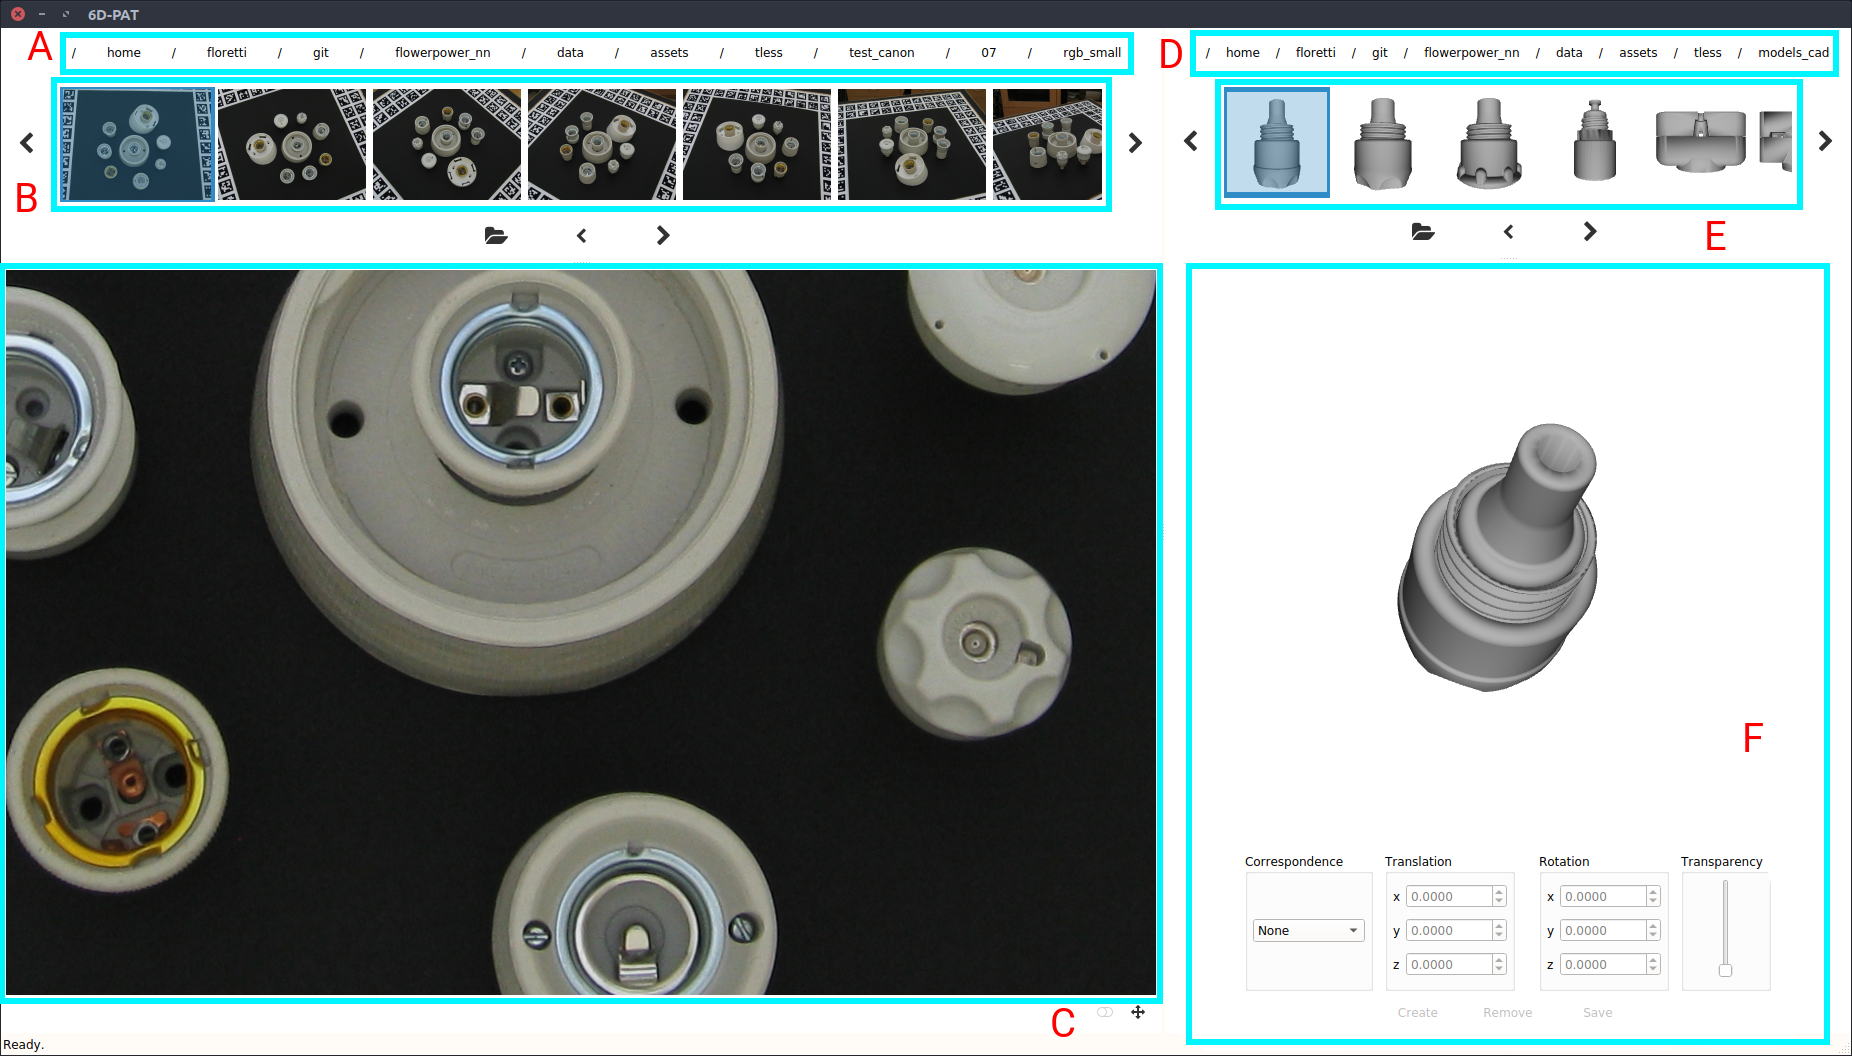
\includegraphics[width=\linewidth]{6dpat_components}
    	\caption{The user interface of the annotation tool 6D-PAT. The data displayed are images and object models from the T-Less dataset. The components marked with a turquoise box are the following ones: \textbf{A}: The full path of the currently selected folder to load images from. \textbf{B}: The gallery showing the images loaded from the selected path. \textbf{C}: The \textit{Correspondence Viewer} shows the image selected in gallery B. The user can click on the image to define the 2D point of a new correspondence. \textbf{D}: The full path of the currently selected folder to load object models from. \textbf{E}: The rendered 3D preview of the object models loaded from the selected path. \textbf{F}: The \textit{Correspondence Editor} shows the object model selected in gallery E. The user can click on the object model to complete the correspondence with the 3D point. the controls at the bottom can be used to edit existing correspondences. Own image.}
    	\label{fig:6dpat_components}
	\end{subfigure}
	\par\bigskip
	\begin{subfigure}[t]{0.47\textwidth}
		\centering
    	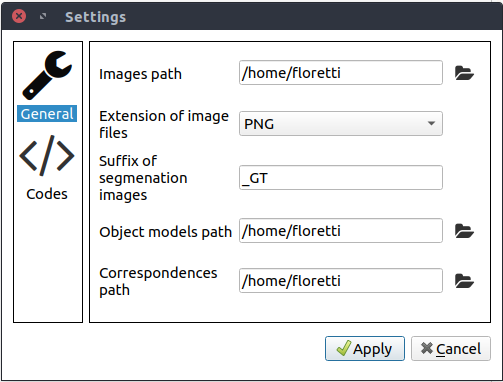
\includegraphics[width=0.8\linewidth]{6dpat_settings}
    	\caption{The settings dialog of 6D-PAT. From here the paths to the images and object models can be set, as well as the segmentation image suffix the image type and the file to write the poses to. Own image.}
    	\label{fig:6dpat_settings}
	\end{subfigure}
	\hfill
	\begin{subfigure}[t]{0.47\textwidth}
	\centering
    	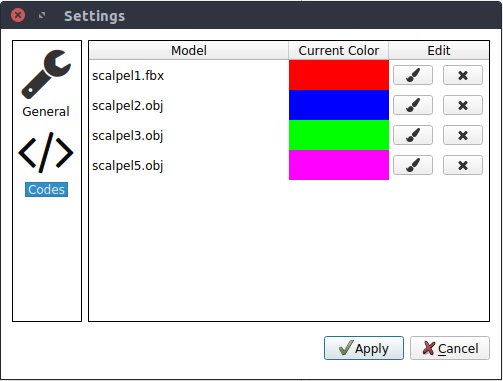
\includegraphics[width=0.8\linewidth]{6dpat_settings_codes}
    	\caption{The settings dialog while editing the colors of the object models in the segmentation images. Own image.}
    	\label{fig:6dpat_settings_codes}
	\end{subfigure}
	\caption{The main view of 6D-PAT as well as the two settings views.}
	\label{fig:6dpat_ui_overview}
\end{figure}

The first step after starting the program is to open the settings (see fig. \ref{fig:6dpat_settings}) and set the path to the images that are to be annotated, as well as the path to the folder that contains the object models that should be used for annotation. 

The folder of the images has to contain a JSON file that holds the camera matrix $K$ for each individual image. If no camera info file exists, a Python script, that is distributed with the neural network, can be used to created approximate camera matrices. The path to the segmentation images (if any) has to be set as well. The program loads the images and the segmentation images and sorts them by the numbers in their filenames and then matches image $I$ at index $j$ with the segmentation image $S$ at index $j$. 

Lastly, the location of the JSON file where the ground-truth poses are to be written to has to be specified. If no such file exists an empty one can be created and selected. If segmentation images are present they are linked to the respective image and can be viewed by activating the toggle at the bottom right corner of the correspondence viewer (the program displaying a segmentation image can be seen in fig. \ref{fig:sfb_segmentation}). 

If required, the colors of the object models in the segmentation images can be set using the settings dialog as shown in fig. \ref{fig:6dpat_settings_codes}. This can reduce the number of displayed tools if many different tools are needed for annotation.

\subsubsection{Correspondence and Pose Creation}

To create a pose an image $I$ has to be selected from gallery B, first. The correspondence viewer C then displays the image. The model $O$ that the image is to be annotated with can be selected from the gallery E. The correspondence editor F shows the selected object model. The user can rotate the object the reach otherwise hidden areas of it. The arrow keys can be used to move the object along the $x$ and $y$ and also, if the shift key is pressed, along the $z$ axis. 

When the object is in an appropriate position, the user can begin to create a correspondence $C$ by clicking on $I$ and this way defining the 2D point $u$ of the correspondence. To complete the correspondence, the object model $O$ has to be clicked at the respective position $p$. This procedure has to be repeated until enough correspondences have been defined to create the new pose $P$. The minimum is 4 correspondences. 

The creation process is shown in fig. \ref{fig:6dpat_correspondence_creation}. More correspondences can make the initial pose more accurate. Clicking the "Create" button at the bottom of the correspondence viewer creates the pose $P$ using the correspondences $C_i$ and OpenCV's \textit{solvePnPRansac} method. The newly created pose is directly selected for editing and can be refined using the controls of the correspondence viewer. After pose refinement it is necessary to click the "Save" button. 

The slider labeled "Transparency" can be used to reduce the object's opacity on the image. After all poses have been annotated successfully the next image can be selected from the gallery B. This operation has to be repeated until the dataset is fully annotated, although intermediate states can be used to train the network already (see chapter \ref{chapter:semi_automatic}).

It is possible to use the neural network to predict poses. This requires a proper setup and training of the network beforehand. The prediction process can be started by clicking the "Predict" button in the lower right corner of the correspondence editor.

\begin{figure}[!tbp]
	\centering
    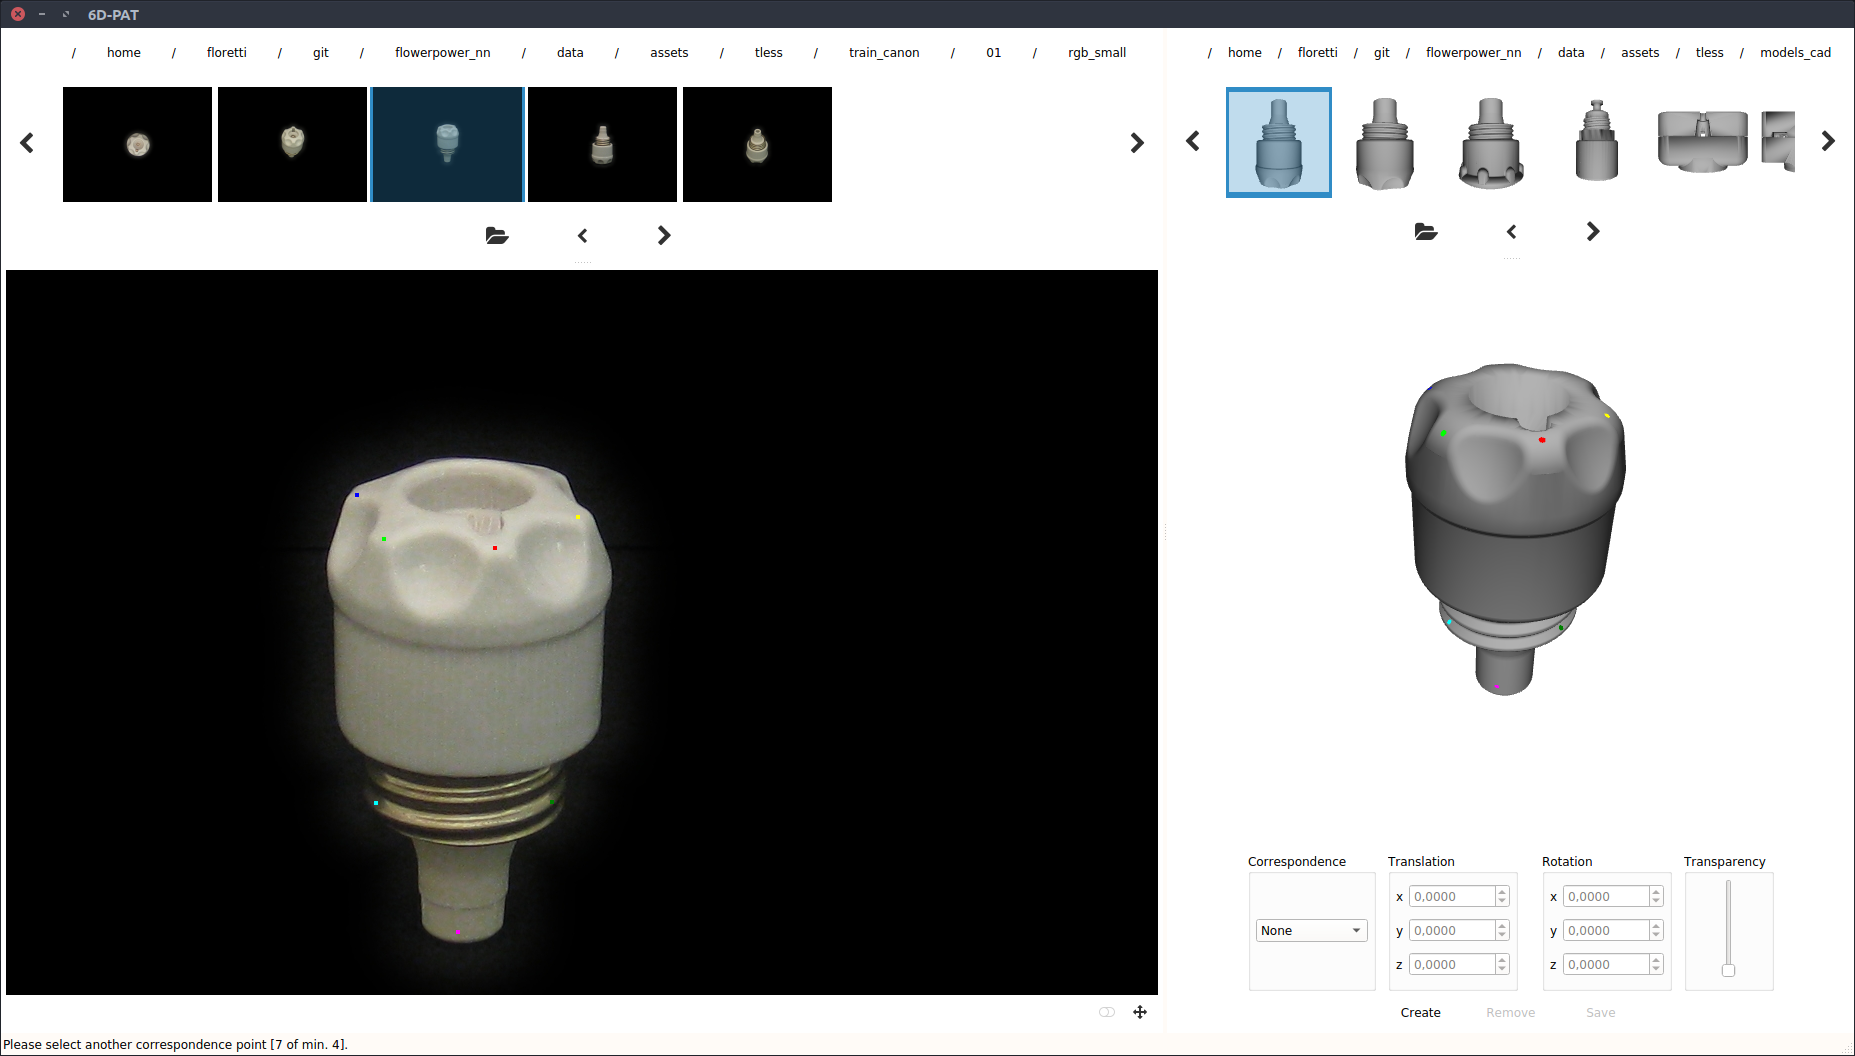
\includegraphics[width=\linewidth]{6dpat_correspondence_creation}
    \caption{The pose creation process by clicking corresponding 2D and 3D points on the displayed image and object model, visualized by the program as colored dots. Own image.}
    \label{fig:6dpat_correspondence_creation}
\end{figure} 

\subsection{Problems \& Difficulties} \label{section:6dpat_difficulties}

\begin{figure}[!tbp]
	\centering
    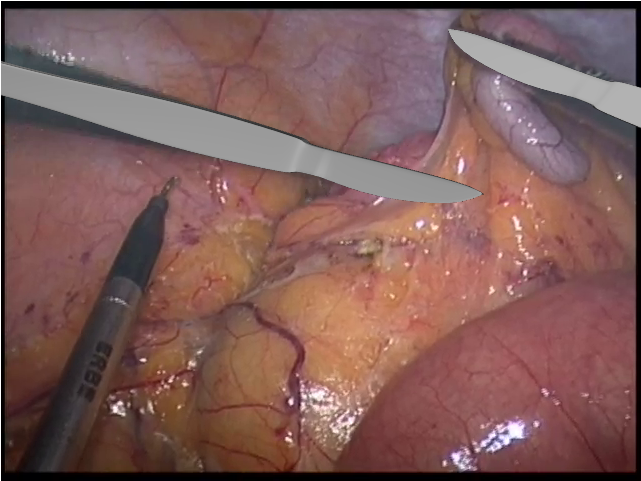
\includegraphics[width=\linewidth]{6dpat_sfb_image}
    \caption{6D-PAT displaying an image from the medical images dataset together with the associated object models. The models are not from datast and thus do not fit the image entirely. Own image.}
    \label{fig:6dpat_sfb_image}
\end{figure} 

\begin{figure}[!tbp]
	\centering
    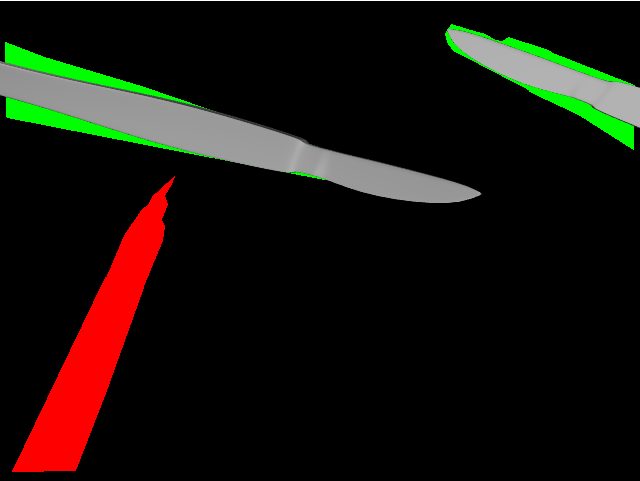
\includegraphics[width=\linewidth]{6dpat_sfb_segmentation}
    \caption{6D-PAT displaying the segmentation image of an image from the medical images dataset. Segmentation images can be viewed by activating the toggle at the bottom right corner of the correspondence viewer, if they are present. Own image.}
    \label{fig:6dpat_sfb_segmentation}
\end{figure} 

During the implementation of the program multiple problems arose and complicated the development process. The most drastic ones are mentioned in this section. Issues contradicting the initial usage patterns and their impact on the final design of the program are explained, as well. \\

One of the major factors that prolong the implementation process was the usage of the only recently released \textit{Qt3D}, which is part of the Qt framework. Qt3D's purpose is to encapsulate graphics programming to increase portability of applications including 3D graphics. The incomplete documentation and unintuitive concepts make it difficult to use without consultation. After more and more complications emerged in the almost completed product the Qt3D framework was deemed unusable and omitted in favor of a native OpenGL implementation. \\

Initially, a desired feature of the program was to present a next unannotated image when the user annotated all poses of an image. This is not feasible for multiple reasons. First of all, a user might still not be content with the poses and might signal that they are finished with the annotation process too early. Thus, it might be disturbing when the program automatically shows the next image. 

The datasets to annotate can also have very distinct characteristics, which require the user to choose the next image personally. For a dataset like T-Less, many images have to be skipped due to their similarity. Intuitively, the more diverse poses are annotated, the better a neural network can be trained. Instead of forcing the user to annotate varying images the motivation should be the sped up annotation process as soon as the neural network is able to make plausible predictions. 

The diversity of kinds of dataset is also the reason why the program does not provide functionality to initialize the next poses based on the ones in the last image. This feature would imply too many assumptions on the dataset and, in the worst case, cause more work for the user. \\

While trying to annotate the medical images dataset it became clear, that proper 3D models are crucial for successful annotation. To temporarily annotate the medical images, 3D surgical tools were downloaded from the internet as a replacement for the missing object models. But having a different shape and also missing the distinctive features of the real objects makes in very difficult to estimate the ground-truth pose. 

It is not clear what the influence of contradicting annotated poses is during training of a network. The author of this work strongly recommends to obtain the correct 3D models before annotating the medical images. The issue of the object models not fitting the segmentation mask can be seen in fig. \ref{fig:sfb_segmentation}. Fig. \ref{fig:sfb_original} shows the actual image and the discrepancy between the models and the pixels belonging to the models. \\

Although Python provides C++ bindings the integration of it into the application is quite involved. This is due to the used development environment being more complex than the one needed for a standard C++ console program. Qt's own makefile generator called \textit{qmake} is distributed with Anaconda (for details on Anaconda see chapter \ref{chapter:semi_automatic}). 

By integrating Python into the application Qt Creator's build system tried to use Anaconda's qmake, which caused the build to fail. Unlike normally, the Qt libraries have to be included explicitly in the project. This requires knowledge of the user which Qt libraries they have installed and further complicates the setup process and demands a computer science specialist. 

Furthermore, the Python binding is not complete yet. Training is not possible and the a deep learning expert has to setup the network and its parameters to enable its usage in the program. The current state of the incorporation of the network is to be seen as a proof of concept that requires further development.

Because the neural network is trained only for one object, the time-intensive (proportional to the overall time needed for inference on one image only) step of loading the trained weights has to be performed each time when running inference for different objects.

\subsection{Future Improvements of 6D-PAT}

To provide an outlook how the program can be improved in the future, some key problems as well as their solutions are listed here. An important feature that should be implemented is moving the object models around on the displayed image by dragging them. It should also be possible to rotate them with the mouse. The initial poses of the models using the clicking procedure are pretty accurate in many cases already. But sometimes, when the camera is looking along an axis of the object directly, it happens that the rotation is far off. The user can correct the poses with the provided controls. But using them takes some skill and time. The describe editing process would profit in terms of time needed per annotation. 

The problem of the time needed for loading the weights of the neural network could be solved by offering an intermediate screen that allows to select many images and the object that is to be annotated. The time of loading the weights gets amortized when running inference for many images. Another possibility is to add a component that allows selection of the weights to be loaded and inference is then only run for the corresponding object. This way a reference to the network with the loaded weights could be held and inference could be run without the loading step.

Two options arise to fully include the neural network in the annotation tool. The first is to complete the Python bridge to support all network operations. It is not possible to automatically set all parameters for the network but the need for a deep learning expert can probably be reduced to a minimum and limited to setting up the network. The other option is to completely re-write the application in Python. The initial intuition that a C++ program offers superior performance over Python is not tenable. Although Python is slower in general Qt bindings for Python allow usage of the C++ components by calling them from Python. The same holds for various OpenGL bindings for Python. The author of this work assumes that there would be no significant  performance loss when using Python as the main language. Including the network is a lot easier when using only Python. An application in Python is also fully portable and experienced users can easily and quickly modify the tool. Although the methods described in chapter \ref{chapter:semi_automatic} are a feasible way of operating the neural network, incorporating the network into the annotation tool would allow inexperienced users to make use of it, too.